\iffalse
Текст текст текст текст текст\\

\section{Название подраздела 1}

\begin{figure}[H]
	\begin{center}
		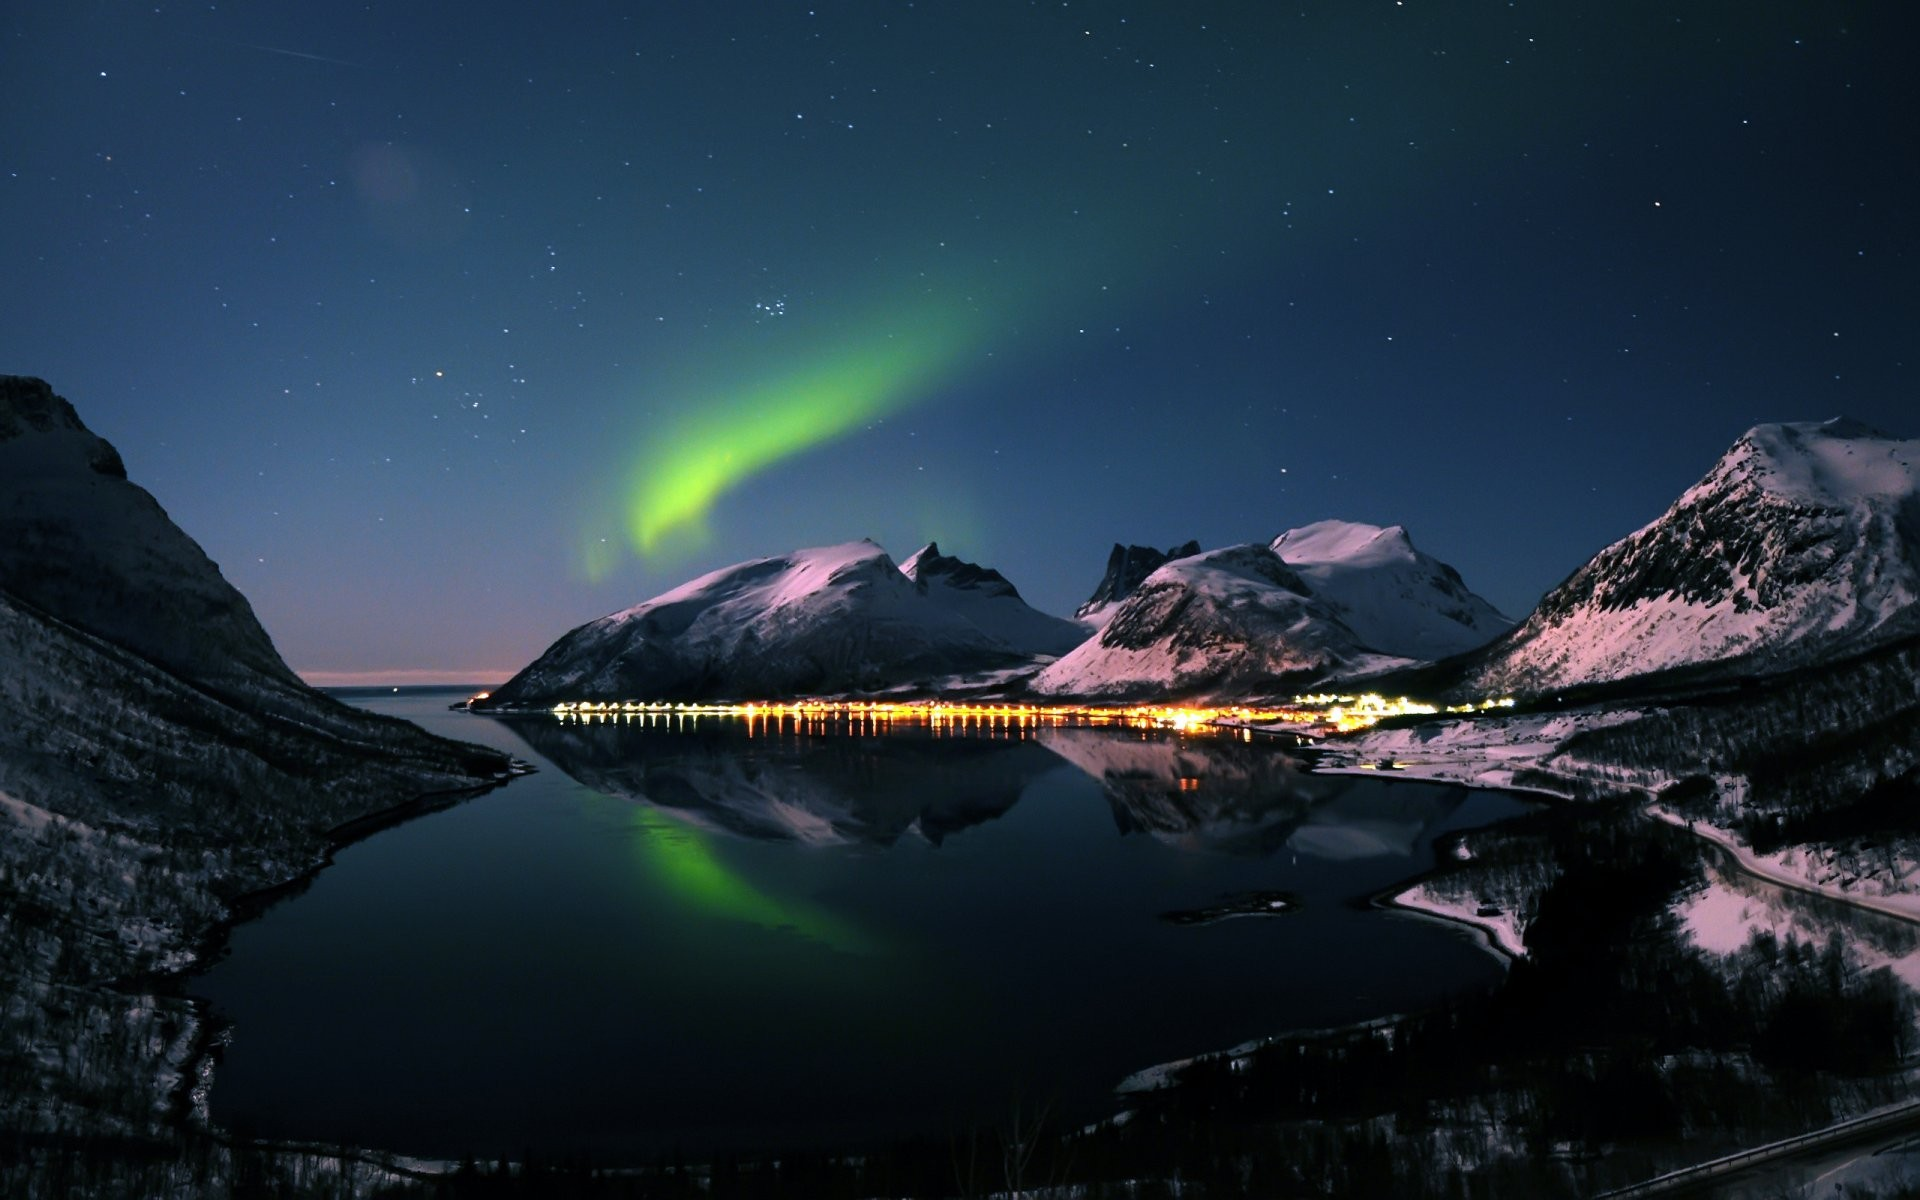
\includegraphics[width=0.7\linewidth]{src/img/img_example.png}
		\caption{Пример вставки изображения}
		\label{fig:img_example}
	\end{center}
\end{figure}

\section{Название подраздела 2}

\begin{center}
	%\resizebox{\textwidth}{!}{
		\begin{tabular}{|c|c|c|}
			\hline
			A1 & B1 & C1 \\ \hline
			A2 & B2 & C2 \\ \hline
		\end{tabular}
		%}
\end{center}
\captionof{table}{Пример вставки таблицы}
\label{tab:tab_example}
\fi
